\subsection{Wellen Allgemein} \ref{sec_wellen_allg}
    {\centering Wellengleichung: \par}
    \begin{minipage}{0.54\linewidth}
        \begin{empheq}[box = \fbox]{align*}
            A(z, t) &= A_0 cos(\omega t - k z)\\
            k &= \frac{2 \pi}{c} \cdot f = \frac{2 \pi}{\lambda}\\
            f &= \frac{1}{T}\\
            \lambda &= \frac{c}{f}\\
            \omega &= 2 \pi f
        \end{empheq}
    \end{minipage}
    \begin{minipage}{0.44\linewidth}
        \begin{scriptsize}
            \begin{empheq}{align*}
                A_0 &= \text{Maximale Amplitude}\\
                \omega &= \text{Kreisfrequenz}\\
                k &= \text{Wellenzahl}\\
                f &= \text{Frequenz}\\
                \lambda &= \text{Wellenlänge}\\
                T &= \text{Periode}\\
                c &= v = \text{Geschwindigkeit der Welle}\\
                &\text{Für Licht in Vakuum: } c = c_0\\
                z &= \text{Abstand zu Ursprung der}\\
                & \text{cos-Funktion zu Zeitpunkt }t_0
            \end{empheq}
        \end{scriptsize}
    \end{minipage}

    \subsubsection{Gruppengeschwindigkeit $v_g$}
    \begin{minipage}{0.69\linewidth}
        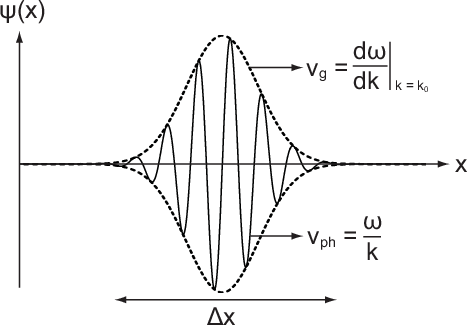
\includegraphics[width = \linewidth]{src/images/gruppengeschwindigkeit.png}
    \end{minipage}
    \begin{minipage}{0.29\linewidth}
        Geschwindigkeit, mit der sich das Wellenpaket fortbewegt
    \end{minipage}
    
    \subsubsection{Reflektion von Wellen}
    Phasensprung bei Welle im Seil mittels Superposition mit einer Welle von der anderen Seite\\
    \begin{minipage}{0.49\linewidth}
        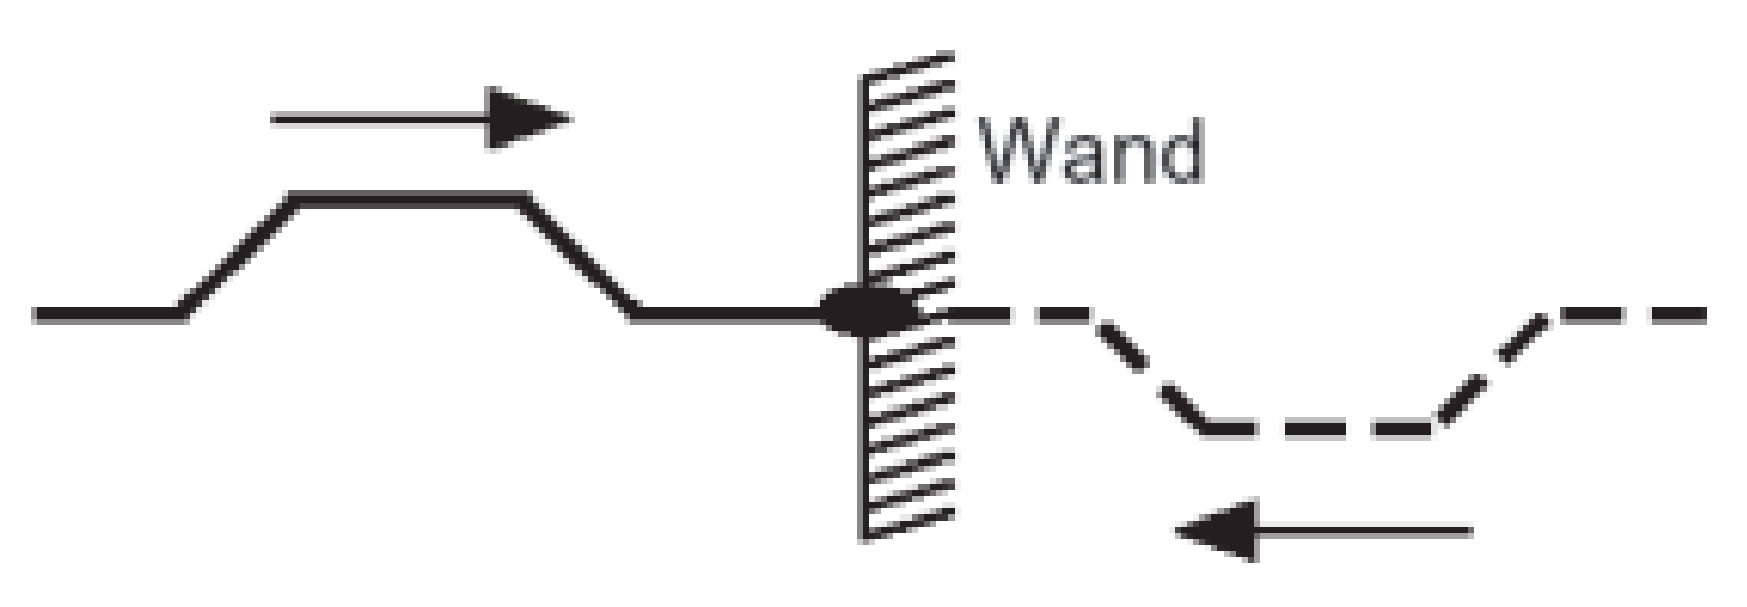
\includegraphics[width = \linewidth]{src/images/welle_superposition_wand.png}
    \end{minipage}
    \begin{minipage}{0.49\linewidth}
        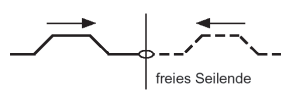
\includegraphics[width = \linewidth]{src/images/welle_superposition_frei.png}
    \end{minipage}

    \subsubsection{Energie von Wellen}

    Intensität einer Welle: Energie
    Potentielle Energie:
    \mathbox{\Delta E_p = \int \vec{F} \vec{dx} = \frac{1}{2} D x_0^2 \text{mit} D = \omega^2 m}
    Kinetische Energie:
    \mathbox{\Delta E_k = \frac{1}{2} \Delta m v^2 \text{mit} v = \omega s}
    $\rightarrow \Delta E_p = \Delta E_k$  

    Energiestromdichte:
    \mathbox{\vec{j_E} = \frac{1}{A} \frac{\Delta E_k}{\Delta t} = \rho_E \vec{v_ph}}